
\begin{yaracode}

import "math"
import "console"
import "time"

rule log_test{
    // output strings !!!
    condition:
       
        console.log("The time now : ", time.now())
        and console.hex("Byte at 0: ", uint8(0))
        and console.hex("Word at 0: ", uint32(0))
        and console.log("")
        and console.hex("Byte at 1: ", uint8(1))
        and console.hex("Word at 1: ", uint32(1))
        and console.log("")
        and console.hex("Byte at 2: ", uint8(2))
        and console.hex("Word at 2: ", uint32(2))
        and console.log("")
        and console.hex("Word at 20: ", uint8(32))
        and console.log("")
        and console.log("The entropy: ", math.entropy( 0, filesize ))
        and console.log("The mode byte: ", math.mode( 0, filesize ))
        and console.log("The percentage of the mode byte: ", math.percentage( math.mode( 0, filesize), 0, filesize ))
        and console.log("The filesize : ", filesize)
        
}

\end{yaracode}
The output when the rule is applied to our malware is like the following
\\

\begin{figure}[H]

    \centering
    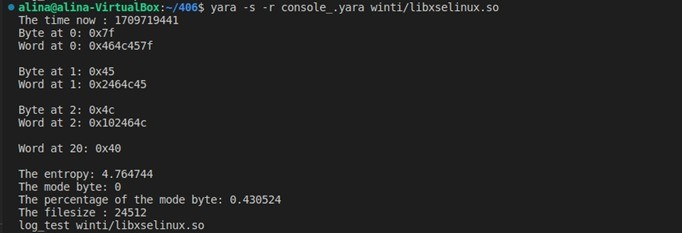
\includegraphics[width=\textwidth]{log.jpeg}
    \caption{Printing in console by Console module}
    \label{fig:file_console}
    
\end{figure}

